% Options for packages loaded elsewhere
\PassOptionsToPackage{unicode}{hyperref}
\PassOptionsToPackage{hyphens}{url}
%
\documentclass[
]{book}
\usepackage{amsmath,amssymb}
\usepackage{iftex}
\ifPDFTeX
  \usepackage[T1]{fontenc}
  \usepackage[utf8]{inputenc}
  \usepackage{textcomp} % provide euro and other symbols
\else % if luatex or xetex
  \usepackage{unicode-math} % this also loads fontspec
  \defaultfontfeatures{Scale=MatchLowercase}
  \defaultfontfeatures[\rmfamily]{Ligatures=TeX,Scale=1}
\fi
\usepackage{lmodern}
\ifPDFTeX\else
  % xetex/luatex font selection
\fi
% Use upquote if available, for straight quotes in verbatim environments
\IfFileExists{upquote.sty}{\usepackage{upquote}}{}
\IfFileExists{microtype.sty}{% use microtype if available
  \usepackage[]{microtype}
  \UseMicrotypeSet[protrusion]{basicmath} % disable protrusion for tt fonts
}{}
\makeatletter
\@ifundefined{KOMAClassName}{% if non-KOMA class
  \IfFileExists{parskip.sty}{%
    \usepackage{parskip}
  }{% else
    \setlength{\parindent}{0pt}
    \setlength{\parskip}{6pt plus 2pt minus 1pt}}
}{% if KOMA class
  \KOMAoptions{parskip=half}}
\makeatother
\usepackage{xcolor}
\usepackage{longtable,booktabs,array}
\usepackage{calc} % for calculating minipage widths
% Correct order of tables after \paragraph or \subparagraph
\usepackage{etoolbox}
\makeatletter
\patchcmd\longtable{\par}{\if@noskipsec\mbox{}\fi\par}{}{}
\makeatother
% Allow footnotes in longtable head/foot
\IfFileExists{footnotehyper.sty}{\usepackage{footnotehyper}}{\usepackage{footnote}}
\makesavenoteenv{longtable}
\usepackage{graphicx}
\makeatletter
\newsavebox\pandoc@box
\newcommand*\pandocbounded[1]{% scales image to fit in text height/width
  \sbox\pandoc@box{#1}%
  \Gscale@div\@tempa{\textheight}{\dimexpr\ht\pandoc@box+\dp\pandoc@box\relax}%
  \Gscale@div\@tempb{\linewidth}{\wd\pandoc@box}%
  \ifdim\@tempb\p@<\@tempa\p@\let\@tempa\@tempb\fi% select the smaller of both
  \ifdim\@tempa\p@<\p@\scalebox{\@tempa}{\usebox\pandoc@box}%
  \else\usebox{\pandoc@box}%
  \fi%
}
% Set default figure placement to htbp
\def\fps@figure{htbp}
\makeatother
\setlength{\emergencystretch}{3em} % prevent overfull lines
\providecommand{\tightlist}{%
  \setlength{\itemsep}{0pt}\setlength{\parskip}{0pt}}
\setcounter{secnumdepth}{5}
\usepackage{booktabs}
\usepackage[]{natbib}
\bibliographystyle{plainnat}
\usepackage{bookmark}
\IfFileExists{xurl.sty}{\usepackage{xurl}}{} % add URL line breaks if available
\urlstyle{same}
\hypersetup{
  pdftitle={Functional Enrichment Workshop},
  pdfauthor={Monash Genomics and Bioinformatics Platform (MGBP)},
  hidelinks,
  pdfcreator={LaTeX via pandoc}}

\title{Functional Enrichment Workshop}
\author{Monash Genomics and Bioinformatics Platform (MGBP)}
\date{Compiled: September 02, 2024}

\begin{document}
\maketitle

{
\setcounter{tocdepth}{1}
\tableofcontents
}
\begin{center}\rule{0.5\linewidth}{0.5pt}\end{center}

\chapter{Getting started}\label{getting-started}

Instructors:

\begin{itemize}
\tightlist
\item
  \textbf{Hossein V Kahrood}

  \begin{itemize}
  \tightlist
  \item
    Monash Genomics and Bioinformatics Platform (MGBP)
  \item
    Lead Instructor
  \item
    \href{mailto:hossein.valipourkahrood@monash.edu}{\nolinkurl{hossein.valipourkahrood@monash.edu}}
  \end{itemize}
\item
  \textbf{Cali Willet}

  \begin{itemize}
  \tightlist
  \item
    Sydney Informatics Hub
  \item
    Lead Instructor
  \item
    \href{mailto:cali.willet@sydney.edu.au}{\nolinkurl{cali.willet@sydney.edu.au}}
  \end{itemize}
\end{itemize}

\section{Summary}\label{summary}

Important links:

\chapter{Overview}\label{overview}

\section{Functional analysis of -Omics data}\label{functional-analysis-of--omics-data}

Workshop 2024

\subsection{General information}\label{general-information}

The workshop covers the bioinformatics concepts and tools available for interpreting a gene list using gene ontology and pathway information. The workshop focuses on the principles and concepts required for analyzing and conducting functional and pathway analysis on a gene list from any organism, although the focus will be on human and model eukaryotic organisms.

\subsection{Course Objectives}\label{course-objectives}

Participants will gain practical experience and skills to be able to:

\begin{itemize}
\tightlist
\item
  Understand basic concepts of functional enrichment analysis;
\item
  Interpret enrichment analysis results;
\item
  Get systems perspective of gene functions;
\item
  Get more information about a gene list;
\item
  Discover what pathways are enriched in a gene list (and use it for hypothesis generation);
\item
  Predict gene function and extend a gene list;
\item
  Follow workflow after the workshop to conduct their own analysis.
\end{itemize}

\subsection{Target Audience}\label{target-audience}

This workshop is intended for biologists working with `-Omics data' (e.g.~RNA-Seq, protein expression and other omics data), who are interested in interpreting large gene/protein lists resulting from their experiments.

\subsection{Setup Requirements}\label{setup-requirements}

This workshop will be delivered online over zoom; you may wish to install the dedicated zoom. Otherwise, no special software installation will required, as we will be using online analysis tools.

\begin{itemize}
\tightlist
\item
  Zoom Link:
\end{itemize}

Links and material will be provided on the day. BYO coffee.

\subsection{Schedule}\label{schedule}

\begin{longtable}[]{@{}lr@{}}
\toprule\noalign{}
Time & Programme \\
\midrule\noalign{}
\endhead
\bottomrule\noalign{}
\endlastfoot
10:30 & Welcome \& Session 1 \\
12:00 & Break \\
12:20 & Session 2 \\
13:30 & Wrap-up \\
\end{longtable}

\subsection{Post-workshop survey}\label{post-workshop-survey}

We appreciate your feedback (both positive and negative !) - please fill out the short post-workshop survey \href{https://docs.google.com/forms/d/e/1FAIpQLSdmWreDIWjVsIR5g22jvcypH8ChFyMJ506HTAIoMIJYzjD-3Q/viewform}{Feedback Survey} in the last 5 mins.

\chapter{Enrichment Statistics}\label{enrichment-statistics}

Enrichment statistics are based on a contingency table like so:

\begin{longtable}[]{@{}
  >{\centering\arraybackslash}p{(\linewidth - 6\tabcolsep) * \real{0.3774}}
  >{\raggedleft\arraybackslash}p{(\linewidth - 6\tabcolsep) * \real{0.2075}}
  >{\raggedleft\arraybackslash}p{(\linewidth - 6\tabcolsep) * \real{0.2830}}
  >{\raggedleft\arraybackslash}p{(\linewidth - 6\tabcolsep) * \real{0.1321}}@{}}
\toprule\noalign{}
\begin{minipage}[b]{\linewidth}\centering
Gene
\end{minipage} & \begin{minipage}[b]{\linewidth}\raggedleft
..in term
\end{minipage} & \begin{minipage}[b]{\linewidth}\raggedleft
..not in term
\end{minipage} & \begin{minipage}[b]{\linewidth}\raggedleft
Total
\end{minipage} \\
\midrule\noalign{}
\endhead
\bottomrule\noalign{}
\endlastfoot
..in gene list & 50 & 100 & 150 \\
..not in gene list (but in background) & 200 & 15900 & 16100 \\
Total & 250 & 16000 & 16250 \\
\end{longtable}

This is based on the 16250 genes that were measured in your experiment.

Note that there might be extra genes that weren't measured these are excluded from the calculations entirely. E.g. There might have been an extra 5000 terms (some of which might have been annotated with the term of interest), making for 21250 \emph{annotated} genes.

\begin{center}\rule{0.5\linewidth}{0.5pt}\end{center}

\section{Interactive Calculator}\label{interactive-calculator}

\href{https://bioinformatics3.erc.monash.edu/rsconnect/content/241/}{\emph{Link to open toy enrichment calculator}}.

This calculates enrichment for a single hypothetical genelist (e.g.~your RNAseq differentially expressed genelist) against a single hypothetical `term' (some set of interesting genes, e.g.~synaptic signaling genes). It makes a Venn diagram and a wordy description of what is being tested.

You can adjust various factors and see their effect on the enrichment p-values.

\begin{quote}
\emph{Note:} This is just a toy calculator for this training, it quite limited. Bonus points if you break it. There are online hypergeometric test or fishers exact test calculators available if you ever need to calculate this directly e.g.~: \url{https://keisan.casio.com/exec/system/1180573201}
\end{quote}

\begin{center}\rule{0.5\linewidth}{0.5pt}\end{center}

\section{Questions}\label{questions}

\begin{enumerate}
\def\labelenumi{\arabic{enumi}.}
\tightlist
\item
  Is it significant at p=0.05?

  Show

  No, corrected pval=0.087
\item
  What about with a smaller background of 5000 genes (e.g.~proteomic datasets)?

  Show

  Even less so - corrected pval=1
\item
  Or, testing against a smaller database of terms; 2000 terms instead of 10000? With the original 16000 gene background.

  Show

  Yes, now corrected pval=0.017
\item
  19 out of 200 differentially expressed genes (9.5\%), need to hit for a 500-gene term (3.1\% of all genes) to be significant at (p=0.048). How many hits would be needed for a more specific 30-gene term?

  Show

  5 hits - 2.5\% of the differentially expressed genes vs 0.19\% of all genes
\end{enumerate}

\chapter{Example Analysis}\label{example-analysis}

\section{SH-SY5Y Differentiation}\label{sh-sy5y-differentiation}

SH-SY5Y is a commonly used neuroblastoma cell line.
With appropriate treatment, it can be induced to differentiate into a `more neuronal' form.
Differentiated cells look quite different, growing thin neurites out from the body of the cell.

\pandocbounded{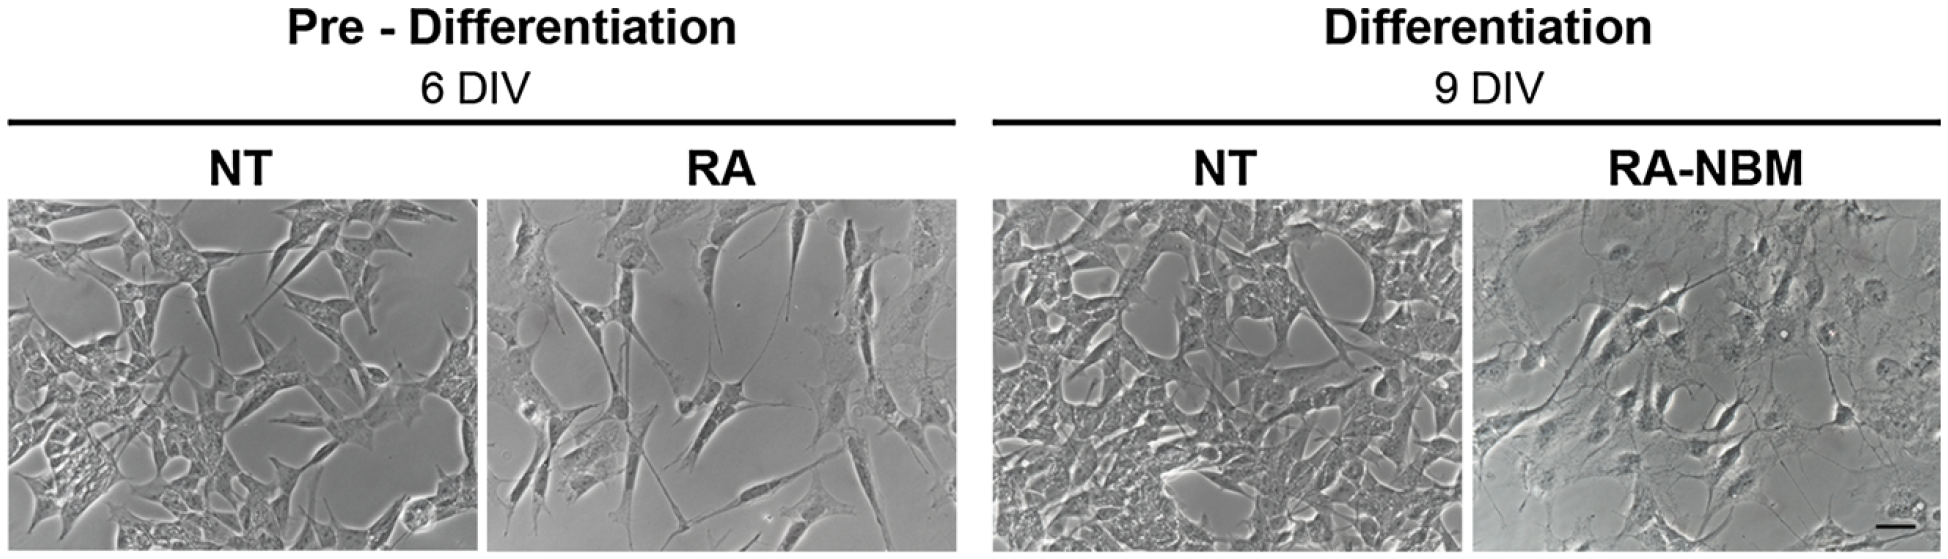
\includegraphics[keepaspectratio]{https://monashbioinformaticsplatform.github.io/enrichment_analysis_workshop/img/shsy5ydiff.png}}

\emph{Image is derived from Figure 4 (Pezzini et al.~2017)}

\section{The question: What pathways are involved in SH-SY5Y Differentiation?}\label{the-question-what-pathways-are-involved-in-sh-sy5y-differentiation}

In their paper \href{https://link.springer.com/article/10.1007\%2Fs10571-016-0403-y}{\emph{Transcriptomic Profiling Discloses Molecular and Cellular Events Related to Neuronal Differentiation in SH-SY5Y Neuroblastoma Cells}} Pezzini et al induced differentiation of the SH-SY5Y Neuroblastoma cell line and measured transcriptomic changes via RNAseq (Pezzini et al.~2017).
They then looked at functional enrichment of differentially expressed genes.

\section{The data : Differentially expressed genes}\label{the-data-differentially-expressed-genes}

The example dataset for today is the RNAseq differential expression results.

They can be accessed via this link:
\url{http://degust.erc.monash.edu/degust/compare.html?code=5b2c7805ab8f8c5f2dc8c72e61b049b0\#?plot=mds}

This has been reanalysed from the published raw data, via the degust tool.

\begin{quote}
Note: Other tools and approaches will have different looking results - but generally you will end up with a table of genes with some measure of statistical confidence.
The methods for functional enrichment analysis should be similar.
\end{quote}

\chapter{Defining the genelist}\label{defining-the-genelist}

Starting from those differential expression results \href{http://degust.erc.monash.edu/degust/compare.html?code=5b2c7805ab8f8c5f2dc8c72e61b049b0\#?plot=mds}{here}, how do we go about getting a genelist to calculate enrichment on?

\section{Activities}\label{activities}

Todays exercise follows the process of getting the differentially expressed gene list using excel. You could use another spreadsheet program, or some may prefer a programming language like R .

\begin{enumerate}
\def\labelenumi{\arabic{enumi}.}
\item
  Download the full table of data from either degust, or the csv file here:
  \href{https://monashbioinformaticsplatform.github.io/enrichment_analysis_workshop/data/Pezzini2016_SHSY5Ycelldiff_DE_table.csv}{Pezzini2016\_SHSY5Ycelldiff\_DE\_table.csv}. Import into excel.
\item
  How many genes are differentially expressed? In these results the FDR Column contains the corrected p-value, and the `differentiated' column shows the log2 fold-change of differentiated cells vs untreated cells (log2(diff)-log2(undiff)); 0 is unchanged, 1 is doubled, -1 is halved.

  \begin{itemize}
  \item
    Significant at 0.01?
  \item
    That's a particularly large number of genes - perhaps not unexpected given how much the cells are changed this experiment. How many significant genes also have 2-fold change in expression?
  \item
    For this workshop, get the genes with a FDR \textless1x10\^{}-4 and 2x fold change. Note that this is a ridiculous threshold - most experiments yeild far less differential expression, but the difference between these two cell conditions is pretty extreme! Typically you would only filter at p\textless0.01 (and occasionally 2-fold change) - you might see 10s to 100s of results. However, this arbitrary threshold gives a more typical number of differentially expressed genes for downstream analysis. An alternative approach could be to take the top 500 genes.
  \end{itemize}

  \{\{\%expand Show\%\}\} There are 4923 differentially expressed genes, 2149 of which have a 2-fold change in expression. With the aggressive filtering - there are 198 genes left \{\{\%/expand\%\}\}
\item
  How many genes are \emph{tested}? This is your background.
  \{\{\%expand Show\%\}\} 14420 genes tested. \{\{\%/expand\%\}\}
\end{enumerate}

\begin{center}\rule{0.5\linewidth}{0.5pt}\end{center}

\section{Common gotcha}\label{common-gotcha}

Can you find SEPT4? Because \href{https://genomebiology.biomedcentral.com/articles/10.1186/s13059-016-1044-7}{\emph{Gene name errors are widespread in the scientific literature}}

You can't revert the gene names automatically (try converting it to text!). You have to avoid it in the first place by importing gene columns as `text' columns in excel. See video from HUGO : \url{https://www.genenames.org/help/faq/\#!/\#tocAnchor-1-25-1}

\begin{center}\rule{0.5\linewidth}{0.5pt}\end{center}

\section{Example}\label{example}

An example excel document showing this filtering process is here: \href{https://monashbioinformaticsplatform.github.io/enrichment_analysis_workshop/data/Pezzini2016_SHSY5Ycelldiff_DE_table_filtering.xlsx}{Pezzini2016\_SHSY5Ycelldiff\_DE\_table\_filtering.xlsx}.

\chapter{Reporting results}\label{reporting-results}

Once we have done an enrichment analysis - how to communicate the results? Like everything - it depends what you need to say. Some examples are below.

\section{In text}\label{in-text}

If you just need to emphasise that the differential expression relates to a condition of interest, you don't need much:

\begin{quote}
Genes differentially expressed after SH-SY5Y cell differentiation were enriched for GO term ``regulation of neurogenesis'', adjusted pval \textless{} 0.01).
\end{quote}

And in the methods:

\begin{quote}
Enrichment calculated for differentially expressed genes with the g:GOSt enrichment tool \href{https://academic.oup.com/nar/article/47/W1/W191/5486750}{(Raudvere et al, 2019)} using a background of tested genes.
\end{quote}

\section{As a table}\label{as-a-table}

For a more complete view, a table of the significant or top \emph{n} terms can be useful. E.g In a supplementary figure

The top 10 enriched GO terms for the differentially expressed genes;

\begin{longtable}[]{@{}
  >{\raggedright\arraybackslash}p{(\linewidth - 8\tabcolsep) * \real{0.4118}}
  >{\raggedright\arraybackslash}p{(\linewidth - 8\tabcolsep) * \real{0.1176}}
  >{\raggedleft\arraybackslash}p{(\linewidth - 8\tabcolsep) * \real{0.1765}}
  >{\raggedleft\arraybackslash}p{(\linewidth - 8\tabcolsep) * \real{0.1078}}
  >{\raggedleft\arraybackslash}p{(\linewidth - 8\tabcolsep) * \real{0.1863}}@{}}
\toprule\noalign{}
\begin{minipage}[b]{\linewidth}\raggedright
\url{GO:BP} Term
\end{minipage} & \begin{minipage}[b]{\linewidth}\raggedright
Term ID
\end{minipage} & \begin{minipage}[b]{\linewidth}\raggedleft
Adjusted p-value
\end{minipage} & \begin{minipage}[b]{\linewidth}\raggedleft
Term Size
\end{minipage} & \begin{minipage}[b]{\linewidth}\raggedleft
Num DE Genes
\end{minipage} \\
\midrule\noalign{}
\endhead
\bottomrule\noalign{}
\endlastfoot
system process & \url{GO:0003008} & 2.90E-04 & 1243 & 45 \\
nervous system development & \url{GO:0007399} & 4.19E-04 & 1985 & 60 \\
regulation of cell development & \url{GO:0060284} & 1.98E-03 & 795 & 33 \\
central nervous system development & \url{GO:0007417} & 2.67E-03 & 805 & 33 \\
regulation of neurogenesis & \url{GO:0050767} & 5.59E-03 & 707 & 30 \\
regulation of nervous system development & \url{GO:0051960} & 5.78E-03 & 790 & 32 \\
regulation of cell differentiation & \url{GO:0045595} & 6.03E-03 & 1471 & 47 \\
multicellular organismal process & \url{GO:0032501} & 2.04E-02 & 5300 & 111 \\
system development & \url{GO:0048731} & 2.88E-02 & 3668 & 85 \\
neurogenesis & \url{GO:0022008} & 4.36E-02 & 1375 & 43 \\
\end{longtable}

\section{As a figure}\label{as-a-figure}

Plots of -log p-value are a popular option for a figure. By taking the exponent of the p-value bigger bars indicate more significance.

For instance, this figure is taken from the \href{https://link.springer.com/article/10.1007\%2Fs10571-016-0403-y}{(Pezzini et al.~2017)} paper.
Note that in this figure shows 2 specifics categories from the IPA (ingenuity) database using the IPA tool (not covered here), so the terms themselves differ.

\pandocbounded{\includegraphics[keepaspectratio]{https://monashbioinformaticsplatform.github.io/enrichment_analysis_workshop/img/NegLogPvalPlot_Pezzini2017.png}}

You can also build on such a plot with number of genes and the like. For an example, see the `bubble' chart produced by a package called pathfindR here: \url{https://www.biostars.org/p/322415/}

\begin{center}\rule{0.5\linewidth}{0.5pt}\end{center}

There are also tools like cluego (a cytoscape plugin) that build enriched terms into a network : \url{http://apps.cytoscape.org/apps/cluego}

\chapter{Resources}\label{resources}

\begin{center}\rule{0.5\linewidth}{0.5pt}\end{center}

Please find a link to today's presentation slides \href{../../enrichment_analysis_2024.pdf}{here}

\begin{center}\rule{0.5\linewidth}{0.5pt}\end{center}

The following tools might be useful for downstream functional analysis; this includes some not covered in todays workshop.

Note that most of these tools do more than just enrichment tests, and some include their own databases.

\section{g:Profiler / g:GOSt}\label{gprofiler-ggost}

\url{https://biit.cs.ut.ee/gprofiler/gost}

The g:GOSt `functional profiling' tool of g:Profiler calculates
It has a clean modern interface and a handy summary of which genes contribute to the enrichment.

\pandocbounded{\includegraphics[keepaspectratio]{https://monashbioinformaticsplatform.github.io/enrichment_analysis_workshop/img/gprofiler.png}}

\section{PANTHER}\label{panther}

\url{http://www.pantherdb.org/}

PANTHER performs overrepresentation tests across multiple databases; Gene ontology, reactome, PANTHER pathways and protein classes. Allows more control over the statistical test used and clearly summarises what was actually done.

\pandocbounded{\includegraphics[keepaspectratio]{https://monashbioinformaticsplatform.github.io/enrichment_analysis_workshop/img/panther.png}}

\section{DAVID}\label{david}

\url{https://david.ncifcrf.gov/}

Via its `functional annotation' tool, DAVID allows you to calculate functional enrichment across a number of databases ; Gene Ontology, KEGG, reactome and others. Reliable, with a slightly clunky interface.

\pandocbounded{\includegraphics[keepaspectratio]{https://monashbioinformaticsplatform.github.io/enrichment_analysis_workshop/img/david.png}}

\section{Enrichr}\label{enrichr}

\url{https://amp.pharm.mssm.edu/Enrichr/}

Enrichr easily calculates enrichment across a wide range of databases. Currently does not allow for a background set.

\pandocbounded{\includegraphics[keepaspectratio]{https://monashbioinformaticsplatform.github.io/enrichment_analysis_workshop/img/enrichr.png}}

\section{Reactome}\label{reactome}

\url{https://reactome.org/}

The core of reactome is the reactome pathways and browser. ALthough other tools use the reactome database, the reactome website provides a means to browse enrichment within the pathway browser view.

\pandocbounded{\includegraphics[keepaspectratio]{https://monashbioinformaticsplatform.github.io/enrichment_analysis_workshop/img/reactome.png}}

\section{Biocyc}\label{biocyc}

\url{https://biocyc.org/}

Biocyc is another suite of tools for enrichment and pathway browsing, which is particularly useful for prokaryotic work. It is licensed, but Monash does have a license.

\pandocbounded{\includegraphics[keepaspectratio]{https://monashbioinformaticsplatform.github.io/enrichment_analysis_workshop/img/biocyc.png}}

\section{STRINGdb}\label{stringdb}

\url{https://string-db.org/}

STRING is not a functional enrichment tool, rather it is a convenient way to explore interactions within a genelist. Results are viewed as an interaction network. Best suited to smaller genelists.

\pandocbounded{\includegraphics[keepaspectratio]{https://monashbioinformaticsplatform.github.io/enrichment_analysis_workshop/img/string.png}}

\section{Gene Ontology}\label{gene-ontology}

\url{http://geneontology.org/}

Gene Ontology (GO) terms are the most widely use set of functional annotations, used by many enrichment tools. The gene ontology resource website itself provides several tools for browsing the GO term hierarchy.

\pandocbounded{\includegraphics[keepaspectratio]{https://monashbioinformaticsplatform.github.io/enrichment_analysis_workshop/img/go.png}}

\section{KEGG}\label{kegg}

\url{https://www.genome.jp/kegg/}

A well known curated pathway database. It is used by many other tools but with a caveat - KEGG moved to a subscription model in 2011, and so enrichment tools need to use the last open release from 2011. However up to date KEGG pathways are browsable directly through their website.

\pandocbounded{\includegraphics[keepaspectratio]{https://monashbioinformaticsplatform.github.io/enrichment_analysis_workshop/img/kegg.png}}

\section{GSEA and MSigDB}\label{gsea-and-msigdb}

\url{http://software.broadinstitute.org/gsea/index.jsp}

The desktop-based GSEA tool is (one of many) gene set enrichment approaches. It uses of gene rankings across all genes rather than hypogeometric or fishers-exact tests of genelist enrichment. MSigDB (Molecular signatures database) is a suite of annotation databases suitable for GSEA analysis.

\pandocbounded{\includegraphics[keepaspectratio]{https://monashbioinformaticsplatform.github.io/enrichment_analysis_workshop/img/gsea.png}}

\section{MetaboAnalyst}\label{metaboanalyst}

MetaboAnalyst is popular among the metabolomics community for statistical, functional and integrative analysis of metabolomics data. It has a feature called \textbf{Functional enrichment analysis}, which performs metabolite set enrichment analysis, metabolic pathway analysis, and pathway activity prediction from MS peaks.

\pandocbounded{\includegraphics[keepaspectratio]{https://monashbioinformaticsplatform.github.io/enrichment_analysis_workshop/img/metaboanalyst.png}}

\section{Cytoscape}\label{cytoscape}

\url{https://cytoscape.org/}

Cytoscape is a desktop-based biological network analysis / visualization tool, rather than a functional enrichment tool (although plugins can change that). It is mentioned here because it is often useful as a next step when you need to create custom figures showing the interactions of an interesting biological pathway.

\pandocbounded{\includegraphics[keepaspectratio]{https://monashbioinformaticsplatform.github.io/enrichment_analysis_workshop/img/cytoscape.png}}

\chapter{End of Session Challenge}\label{end-of-session-challenge}

\section{Dr Dodge's Experiment}\label{dr-dodges-experiment}

There's quite a few ways you can calculate functional enrichment - so there's always a risk of \href{https://bitesizebio.com/31497/guilty-p-hacking/}{p-hacking}, whether accidental or deliberate.

\emph{So lets go deliberate\ldots{}}

Dr Dodge is convinced that your experiment should turn out with relevance to GO term `segmentation' - but p=0.06! But they \emph{must} be significant, the paper needs be submitted by Friday!

What hacky and statistically questionable approaches could you apply to call these results ``significant''?

\chapter{Feedback}\label{feedback}

We appreciate your feedback (both positive and negative !) - please fill out the short post-workshop survey \href{https://docs.google.com/forms/d/e/1FAIpQLSdmWreDIWjVsIR5g22jvcypH8ChFyMJ506HTAIoMIJYzjD-3Q/viewform}{Feedback Survey}

  \bibliography{book.bib,packages.bib}

\end{document}
